% !TEX program = uplatex
% !TEX root = main.tex

\documentclass[Journal,letterpaper,InsideFigs,NoLineNumbers]{ascelike-new}

% Japanese manuscripts should be compiled with LuaLaTeX.
\usepackage[dvipdfmx]{graphicx}
\usepackage{booktabs}
\usepackage{array}
\usepackage[dvipdfmx,colorlinks=true,citecolor=black,linkcolor=black,urlcolor=blue]{hyperref}
\usepackage{pxjahyper}

\newcommand{\argmin}{\mathop{\rm arg~min}\limits}
\newcommand{\E}{\mathrm{E}}

\title{広域連携による橋梁群の維持管理最適化に向けた\\地域分割と集約効果の定量分析}

\author{
福山 峻一\thanks{非会員，東北大学大学院工学研究科（〒980-8579 宮城県仙台市青葉区荒巻字青葉6-6）E-mail: fukuyama.shunichi.p3@dc.tohoku.ac.jp}\\
水谷 大二郎\thanks{正会員，東北大学大学院工学研究科 准教授（〒980-8579 宮城県仙台市青葉区荒巻字青葉6-6）E-mail: daijiro.mizutani.a5@tohoku.ac.jp}
}

%\NameTag{Fukuyama}

\begin{document}

\maketitle

\begin{abstract}
本研究は，橋梁群の効率的な維持管理を目的とした地域分割最適化問題について検討する．老朽化インフラの増加と担い手不足への対応として，国土交通省が推進する「地域インフラ群再生戦略マネジメント（群マネ）」では，面的・群的視点に基づく広域的な維持管理体制の構築が求められている．本研究では，広域連携エリア内での橋梁補修の同時発注を前提とし，確率的劣化の下で計画期間中に発生する契約件数と，連携範囲の広さを考慮し，そのバランスを最適化するモデルを構築する．さらに，実橋梁データを用いた数値実験により，地域分割と集約効果の特性を分析する．本研究は，群マネの有効性を定量的に評価し，最適な広域連携のあり方を検討するうえで有用な数理的基盤を提供する．
\end{abstract}

\begin{center}
\textbf{Keywords:} districting optimization, infrastructure asset management,
contract bundling, evidence-based policymaking (EBPM)
\end{center}

\section{Introduction}

複数の橋梁補修案件を単一契約にまとめる契約バンドリング（contract bundling）は，個別に発注される複数の案件を一つの契約単位に集約する手法である．米国連邦道路局（Federal Highway Administration: FHWA）は，類似案件のバンドリングが，規模の経済によるコスト削減や調達手続の効率化に寄与するとしている\cite{fhwafactsheet}．本研究では，これらの効果のうち，補修需要をより少ない契約単位に集約できる可能性に着目する．

バンドリングの機会は，契約対象とし得る範囲内で，同じ期間に補修を必要とする橋梁がどの程度発生するかに依存する．日本では，市区町村がそれぞれの管理する橋梁について補修工事を発注しているため，同一契約に含め得る橋梁の範囲は，原則として各主体の管理区域に限定される．このため，管理橋梁数が少ない主体ほど，同一期間に発生する補修需要を一つの契約に集約する機会が限られる．また，地理的に近接する橋梁であっても，管理主体が異なれば，通常は同一契約の対象とならない．

この問題への対応として，複数の管理主体が行政界を越えて連携し，橋梁群を一体的に管理・発注することが考えられる．米国Nebraska州では，個々の郡では橋梁バンドリングの便益を十分に得られない場合があることから，複数郡が行政界を越えて橋梁を一つの事業に集約する取組が実施されている\cite{fhwa2019}．

日本では，国土交通省が「地域インフラ群再生戦略マネジメント（群マネ）」を推進し，自治体の枠を越えた広域連携をその一類型として示している\cite{mlit2025gunmane}．

しかし，複数自治体の橋梁を一体的に管理・発注する場合に，どのように管理エリアを設計すれば，地理的制約の下で期待契約件数を最小化できるかは，明らかになっていない．

この問いは，インフラの確率的維持管理，地域分割，道路インフラ事業の契約バンドリングという三つの研究領域にまたがる．インフラ維持管理研究では，確率的な劣化・故障過程を維持管理方針や施設配置の最適化に組み込む方法が研究されてきた\cite{nakazato2023,mizutani2025}．地域分割研究では，地理的な基本単位を複数の地区へ編成するための方法が体系的に研究されてきた\cite{kalcsics2019}．一方，道路インフラ分野の契約バンドリング研究は，あらかじめ選定された事業群から契約ロットを構成する方法を扱っている\cite{qiao2026}．しかし，確率的に発生する橋梁補修需要と契約バンドリングを結び付け，管理エリアの設計問題として扱う枠組みは，確認した範囲では示されていない．

本研究は，確率的劣化に伴う補修需要と契約バンドリングルールを統合した地域分割最適化モデルを構築し，広域連携による契約集約効果を定量的に評価することを目的とする．

本研究の主な貢献は以下の3点である．

\begin{itemize}
\item \textbf{確率的補修需要，契約バンドリング，地域分割の統合的定式化．} 確率的維持管理，契約バンドリング，地域分割として個別に扱われてきた三つの問題を，橋梁補修の管理エリア設計という一つの最適化問題として統合する．
\item \textbf{橋梁劣化データから調達評価への接続．} 点検データからマルコフ推移確率を推定し，補修需要の発生確率を導出するとともに，地域内橋梁数 $N$ と一契約当たりの同時発注上限 $L$ を引数とする期待契約件数の閉形式 $f(N,L)$ を構築する．これにより，確率的な補修需要を契約集約効果の評価指標へ変換し，地域分割最適化の目的関数に組み込む．
\item \textbf{実橋梁データに基づく広域連携効果の定量評価．} 宮城県内の橋梁データを用いて，管理橋梁数，同時発注上限，地域数および距離制約が期待契約件数に与える影響を体系的に分析し，現行の管理単位との比較を通じて契約集約効果を示す．
\end{itemize}

\section{Literature Review}

橋梁や道路を対象とした契約バンドリングに関する研究では，複数事業を一つの契約に集約することの効果と，事業を束ねる際の判断基準が検討されてきた．Qiao\cite{qiao2019}は，インディアナ州の道路・橋梁プロジェクトを対象に，バンドルが単価，工期，入札者数などに与える影響を統計的に分析した．Assaf and Assaad\cite{assaf2023}およびAssaf et al.\cite{assaf2024}は，実際のインフラ事業の分析を通じて，地理的近接性，工種や規模の類似性，事業時期の整合性など，バンドリング戦略に影響する意思決定要因を抽出・体系化した．これらの研究はバンドリングの効果や判断要因を明らかにしているが，将来発生する補修需要をどのような管理範囲の下で集約するかという問題は扱っていない．

契約ロットの構成を明示的な意思決定問題として扱う研究も行われている．Qiao et al.\cite{qiao2026}は，道路工事プロジェクト群を組合せ最適化問題として定式化し，貪欲ヒューリスティックによってバンドリング戦略を導出した．しかし，同研究では候補となるプロジェクトリストがあらかじめ与えられており，補修需要の確率的な発生過程と管理エリアの設計は意思決定の対象に含まれない．また，空間的なグループ化の効果に着目したGooijer\cite{gooijer2024}は，オランダの橋梁約85,000橋を対象に複数のクラスタリング戦略をシミュレーションで比較したが，分析対象はあらかじめ定義されたクラスタ戦略であり，契約集約効果を評価しながらクラスタ自体を形成する最適化ではない．このように，既存のバンドリング研究は，所与の事業群から契約ロットを構成する問題や，所与のクラスタ戦略の効果を主な対象としている．

これに対して，管理エリア自体の設計に関係する研究領域として，地域分割（districting）問題がある．地域分割問題では，地理的な基本単位を複数の地区へ編成する方法が，行政計画，選挙区割り，物流配送などの分野で研究されてきた．Kalcsics and Rios-Mercado\cite{kalcsics2019}は，均衡性，接続性，コンパクト性などの代表的な地区設計基準と，それらを考慮した数理的手法を体系的に整理している．Webster\cite{webster2013}は政治区割りを対象に，人口均等性，コンパクト性，連続性，利害共同体の維持といった評価基準を検討した．また，Novaes et al.\cite{novaes2010}は物流配送を対象とする連続的な地域分割モデルを構築し，Power Voronoi図を用いて地理的障害を考慮した分割を示した．これらの研究は，地理的条件や地区間の均衡を考慮して空間的な地区を設計する方法を提供するが，地区内で確率的に発生する橋梁補修需要や，その需要を契約として集約した場合の期待契約件数を評価基準としていない．

また，本研究では，将来の補修需要を確率的に扱う必要がある．確率的な劣化・故障過程をインフラ維持管理上の意思決定に組み込む研究として，Nakazato et al.\cite{nakazato2023}は，ライフサイクルコストと年度間費用の変動を考慮した補修方針の最適化を扱っている．Mizutani et al.\cite{mizutani2025}は，道路施設の故障過程を考慮した補給部品配置を，連続近似を用いて最適化している．これらの研究は，不確実な劣化・故障過程を意思決定モデルに組み込んでいるが，補修需要の契約集約効果や管理エリアの設計は対象としていない．

以上の研究群は，それぞれ契約ロットの構成，管理エリアの空間設計，補修需要の不確実性を扱ってきた．しかし，これらを結び付け，確率的に発生する橋梁補修需要と契約バンドリングルールから期待契約件数を導出し，管理エリアの設計問題に組み込む枠組みは，確認した範囲では示されていない．本研究は，確率的な補修需要を契約集約効果の評価指標へ変換し，地理的制約の下で期待契約件数を最小化する管理エリアの空間構成を求める点に新規性がある．

\section{Methodology}

\subsection{Problem Setting and Evaluation Metric}

本研究では，複数自治体が管理する橋梁を行政界にかかわらず複数の管理エリアへ割り当て，各エリアで発生する橋梁補修需要を契約バンドリングによって集約する状況を考える．本研究の目的は，確率的に発生する補修需要について，管理エリアの空間構成が契約バンドリングの機会と年間期待契約件数に与える影響を評価することである．また，過度な広域化を避けるため，同一エリアに含まれる橋梁間の最大距離に上限を設ける．

モデルは，確率的補修需要，契約バンドリングルールおよび地域分割最適化の三つの要素から構成される．はじめに，点検データから推定したマルコフ推移確率行列を用いて，単一橋梁の年間補修需要発生確率を算定する．次に，エリア内で補修対象となる橋梁数の確率分布と，一契約に含められる橋梁数の上限から，エリア内橋梁数に応じた年間期待契約件数を求める．最後に，その期待値を目的関数として，距離制約の下で橋梁の地域割当を最適化する．

期待契約件数は，管理エリアの変更によって補修需要をどの程度少ない契約単位へ集約できるかを表す．したがって，その減少は契約集約機会の増加を意味するが，施工費の削減や規模の経済による単価低下を直接表すものではない．本モデルは個別契約を予測するものではなく，管理エリアの空間構成が契約集約の機会に与える影響を比較するためのモデルである．

\subsection{Stochastic Repair Demand and Contract Bundling}

\subsubsection{Deterioration Model}

橋梁の健全度は，離散的な状態間を時間とともに推移する確率過程として表す．健全度の状態空間を \(\{1,\ldots,m\}\) とし，状態番号が大きいほど劣化が進行しているものとする．点検前後の健全度と点検間隔から，津田ら\cite{tsuda2005}のマルコフ劣化ハザードモデルを用いて1年間の推移確率行列 \(P\) を推定する．

最大劣化状態 \(m\) を補修対象状態とし，状態 \(m\) に到達した橋梁は補修後に状態1へ回復すると仮定する．補修前の劣化過程を表す推移確率行列 \(P\) を，非補修状態間の推移行列 \(T\) と，非補修状態から補修状態への推移確率ベクトル \(r\) を用いて，
\[
P=
\left(
\begin{array}{cc}
T & r\\
0 & 1
\end{array}
\right)
\]
と表す．補修による状態1への回復を組み込むと，補修状態を除いた更新過程の推移確率行列は，
\[
\widetilde{P}=T+re_1^{\mathsf T}
\]
となる．ここで，\(e_1=[1,0,\ldots,0]^{\mathsf T}\) は状態1を表す単位ベクトルである．\(\widetilde{P}\) の定常分布 \(\pi\) は，\(\pi\widetilde{P}=\pi\) および \(\pi\mathbf{1}=1\) を満たし，
\[
\pi=
\frac{e_1^{\mathsf T}(I-T)^{-1}}
{e_1^{\mathsf T}(I-T)^{-1}\mathbf{1}}
\]
と表される．この定常分布は，補修状態への到達後に状態1へ回復する更新過程において，橋梁が各非補修状態に存在する長期的な割合を表す．したがって，定常状態において単一橋梁に補修需要が発生する年間確率 \(q\) は，
\[
q=\pi r
\]
によって与えられる．

\subsubsection{Contract Bundling Rule}

地域 \(k\) に含まれる橋梁数を \(N_k\) とする．各橋梁が同一の年間補修需要発生確率 \(q\) を持ち，互いに独立に補修対象になると仮定すると，地域 \(k\) において1年間に補修対象となる橋梁数 \(X_k\) は，
\[
X_k\sim\mathrm{Binomial}(N_k,q)
\]
に従う．したがって，補修対象橋梁数が \(n\) 本となる確率は，
\[
\Pr(X_k=n)
=
{N_k\choose n}q^n(1-q)^{N_k-n}
\]
である．

一契約に含められる橋梁数の上限を \(L\) とする．同一年度かつ同一地域内で発生した補修需要を，上限 \(L\) まで同一契約に含められると仮定すると，補修対象橋梁が \(n\) 本の場合に必要となる契約件数 \(C(n;L)\) は，
\[
C(n;L)=
\left\{
\begin{array}{ll}
0, & n=0,\\
\left\lceil n/L\right\rceil, & n\geq 1
\end{array}
\right.
\]
となる．ここで，\(\lceil n/L\rceil\) は \(n/L\) 以上の最小の整数を表す天井関数である．\(L=1\) は各橋梁を個別に発注する場合を表し，\(L>1\) は最大 \(L\) 橋まで同一契約に含められる場合を表す．\(L\) は実際の契約規模を一意に定める値ではなく，契約バンドリングの許容範囲を表すシナリオパラメータである．

\subsubsection{Expected Number of Contracts}

以上より，橋梁数 \(N_k\) の地域における年間期待契約件数は，
\[
f(N_k,L)
=
\E[C(X_k;L)]
=
\sum_{n=0}^{N_k}
{N_k\choose n}q^n(1-q)^{N_k-n}
\left\lceil\frac{n}{L}\right\rceil
\]
で与えられる．ただし，\(n=0\) の項は0とする．

\subsection{Districting Optimization Model}

\subsubsection{Notation}

橋梁の集合を \(\mathcal{I}\)，\(M\) 個の管理エリアの集合を \(\mathcal{K}=\{1,\ldots,M\}\) とし，橋梁を \(i,j\in\mathcal{I}\)，管理エリアを \(k\in\mathcal{K}\) で表す．橋梁 \(i\) と \(j\) の地理的距離を \(d_{ij}\) とする．橋梁 \(i\) を管理エリア \(k\) に割り当てるとき1となる二値変数を \(x_{ik}\) とする．

\subsubsection{Objective Function and Distance Constraint}

本研究の地域分割では，年間期待契約件数と管理エリア内の地理的な広がりの両方を考慮する必要がある．地域分割 \(x\) の下での年間期待契約件数を
\[
Z(x)=\sum_{k\in\mathcal{K}}f(N_k,L)
\]
とし，同一管理エリアに含まれる橋梁間距離の最大値を
\[
R(x)
=
\max\left\{d_{ij}\mid i,j\in\mathcal{I},\ i<j,\ x_{ik}=x_{jk}=1,\ k\in\mathcal{K}\right\}
\]
とする．ただし，橋梁を1橋のみ含む管理エリアではエリア内最大距離を0とする．

両者を同時に考慮する方法として，まず，次の重み付き和による定式化が考えられる．
\[
\min_x\quad Z(x)+\alpha R(x)
\]
ここで，\(\alpha\) は期待契約件数と距離との相対的な重要度を表す重みである．しかし，\(Z(x)\) の単位は契約件数，\(R(x)\) の単位は距離であるため，\(\alpha\) には両者を換算する役割が必要となり，その値を実務的に解釈して設定することは容易ではない．

そこで本研究では，距離を目的関数に含めず，許容可能なエリア内最大距離 \(D\) を上限として与える制約型の定式化を採用する．すなわち，
\[
\begin{array}{ll}
\displaystyle \min_x & Z(x),\\
\mathrm{s.t.} & R(x)\leq D
\end{array}
\]
とする．\(D\) を複数の値に変化させることで，地理的な広がりの許容範囲と期待契約件数との関係を，単位の異なる指標間の換算を置かずに評価する．

距離制約を簡潔に記述するため，距離が \(D\) を超える橋梁ペアの集合を
\[
\mathcal{E}_D
=
\{(i,j)\in\mathcal{I}\times\mathcal{I}\mid i<j,\ d_{ij}>D\}
\]
と定義する．

\subsubsection{Mathematical Formulation}

地域分割最適化問題を次のように定式化する．
\[
\begin{array}{lll}
\min_{x,N}\quad
& Z=\displaystyle\sum_{k\in\mathcal{K}}f(N_k,L), & \\
\mathrm{s.t.}\quad
& N_k=\sum_{i\in\mathcal{I}}x_{ik}
& \forall k\in\mathcal{K}, \\
& \sum_{k\in\mathcal{K}}x_{ik}=1
& \forall i\in\mathcal{I}, \\
& N_k\geq 1
& \forall k\in\mathcal{K}, \\
& x_{ik}+x_{jk}\leq 1
& \forall (i,j)\in\mathcal{E}_D,\ \forall k\in\mathcal{K}, \\
& x_{ik}\in\{0,1\}
& \forall i\in\mathcal{I},\ \forall k\in\mathcal{K}, \\
& N_k\in\{1,\ldots,|\mathcal{I}|\}
& \forall k\in\mathcal{K}.
\end{array}
\]

目的関数は，管理エリアごとの年間期待契約件数の総和を最小化する．各制約の役割は次のとおりである．
\begin{itemize}
\item 第1制約は，管理エリア \(k\) に含まれる橋梁数 \(N_k\) を定義する．
\item 第2制約は，各橋梁をいずれか一つの管理エリアに割り当てる．
\item 第3制約は，各管理エリアに少なくとも1橋を割り当てる．
\item 第4制約は，\(\mathcal{E}_D\) に含まれる橋梁ペアを同一の管理エリアに割り当てず，各エリア内の最大橋梁間距離を \(D\) 以下に制限する．
\end{itemize}

\subsection{Scenario Parameters}

距離上限 \(D\) は，管理エリアの地理的な広がりの許容範囲を表すシナリオパラメータとして与える．橋梁間距離 \(d_{ij}\) には，橋梁の位置座標に基づく2地点間の大円距離を用いる．

地域数 \(M\) は，実務上の管理体制，契約主体および意思決定の単位等に関係するため，期待契約件数のみから一意に定めることはできない．そこで本研究では，\(M\) を外生的なシナリオパラメータとして与え，複数の \(M\) を比較することで，管理単位の数と契約集約効果との関係を評価する．同時発注上限 \(L\) についても複数の値を設定し，バンドリング可能な契約規模が結果に与える影響を確認する．

\subsection{Assumptions and Scope}

本モデルの評価範囲は，管理エリアの空間構成が，確率的に発生する橋梁補修需要を少ない契約単位へ集約できる可能性に及ぼす影響までとする．この関係を明確にするため，以下を仮定する．
\begin{enumerate}
\item 各橋梁は共通の年間補修需要発生確率 \(q\) を持ち，補修需要は橋梁間で独立に発生する．
\item 同一年度かつ同一地域内で発生した補修需要は，工種や施工条件にかかわらず，上限 \(L\) まで同一契約に含められる．
\item 管理エリアの地理的な広がりは，エリア内の最大橋梁間距離によって表す．
\item 地域数 \(M\) は外生的に与える．また，橋梁を点として扱い，地域間の橋梁数の均衡や面的な区域の連続性は制約しない．
\end{enumerate}

したがって，本モデルによって得られる地域分割は，補修需要の契約集約という観点から管理エリアの候補を示すものであり，実際の共同発注区域を直接決定するものではない．

\section{Numerical Experiments}

\subsection{Data and Preprocessing}

本章では，前章で構築したモデルを，宮城県内の6市町が管理するRC橋322橋へ適用する．劣化推移確率の推定には，全国道路施設点検データベースから抽出した宮城県内のRC橋5,525橋と，道路メンテナンス年報に収録された点検履歴を用いる\cite{roadstructuresdb,roadmaintenance}．地域分割最適化の対象は，七ヶ宿町，白石市，蔵王町，川崎町，村田町および大河原町が管理する322橋である．Figure~\ref{fig:study_area}に対象地域と橋梁位置を示す．現行の管理区分では，これら6市町がそれぞれの橋梁を管理しており，行政界が近接する橋梁群の発注単位を分けている．

\begin{figure}[htbp]
\centering

\includegraphics[width=0.82\linewidth]{figures/study_area.png}
\caption{Distribution of 322 RC bridges in the six municipalities.}
\label{fig:study_area}
\end{figure}

対象6市町ごとに遷移確率を推定するには観測数が限られるため，同一の都道府県内で同じ点検制度の下にあるRC橋全体から，共通の年間推移確率を推定した．この共通の確率を対象322橋へ適用することで，劣化特性の地域差を捨象し，管理エリアの空間構成が契約集約機会に与える影響に焦点を当てる．

点検履歴による連続する健全度判定の組から遷移観測を作成した．前章で示したマルコフ劣化ハザードモデルは，遷移前後の健全度とその間の経過年数を用いて年間推移確率を推定する．そこで，架設年が得られる橋梁については，架設時の健全度をIと仮定した記録を最初の点検記録の前に追加し，架設から初回点検までの遷移も推定に用いた．健全度が改善する観測は，補修・更新の実施または点検判定の基準・解釈の差異を反映し，単調な劣化過程の仮定と整合しないため除外した．あわせて，30年を超える点検間隔の観測を除外した．

Table~\ref{tab:transition_counts}に，IVを統合する前の健全度遷移の集計を示す．日本の道路橋定期点検では，健全度IIIは早期に措置を講ずべき状態，IVは緊急に措置を講ずべき状態に分類される\cite{mlit2014inspection}．本研究では，いずれも補修需要が発生した状態として扱うため，推定前にIVをIIIへ統合し，I，IIおよびIIIからなる3状態モデルを用いた．Figure~\ref{fig:inspection_interval}は，推定に用いた点検間隔の分布である．平均点検間隔は6.46年，中央値は5年であった．日本では2014年7月以降，橋梁の定期点検は5年に1回の頻度を基本としているが，本データには制度導入前の点検履歴と，架設から初回点検までの遷移も含まれるため，平均値は5年を上回る\cite{mlit2014inspection}．

\begin{table}[htbp]
\centering
\caption{Counts of observed condition-state transitions ($n=7{,}628$).}
\label{tab:transition_counts}
\begin{tabular}{lrrrr}
\toprule
 & \multicolumn{4}{c}{To} \\
\cmidrule(lr){2-5}
From & I & II & III & IV \\
\midrule
I & 949 & 1323 & 82 & 0 \\
II & 0 & 4693 & 372 & 2 \\
III & 0 & 0 & 203 & 2 \\
IV & 0 & 0 & 0 & 2 \\
\bottomrule
\end{tabular}
\end{table}

\begin{figure}[htbp]
\centering
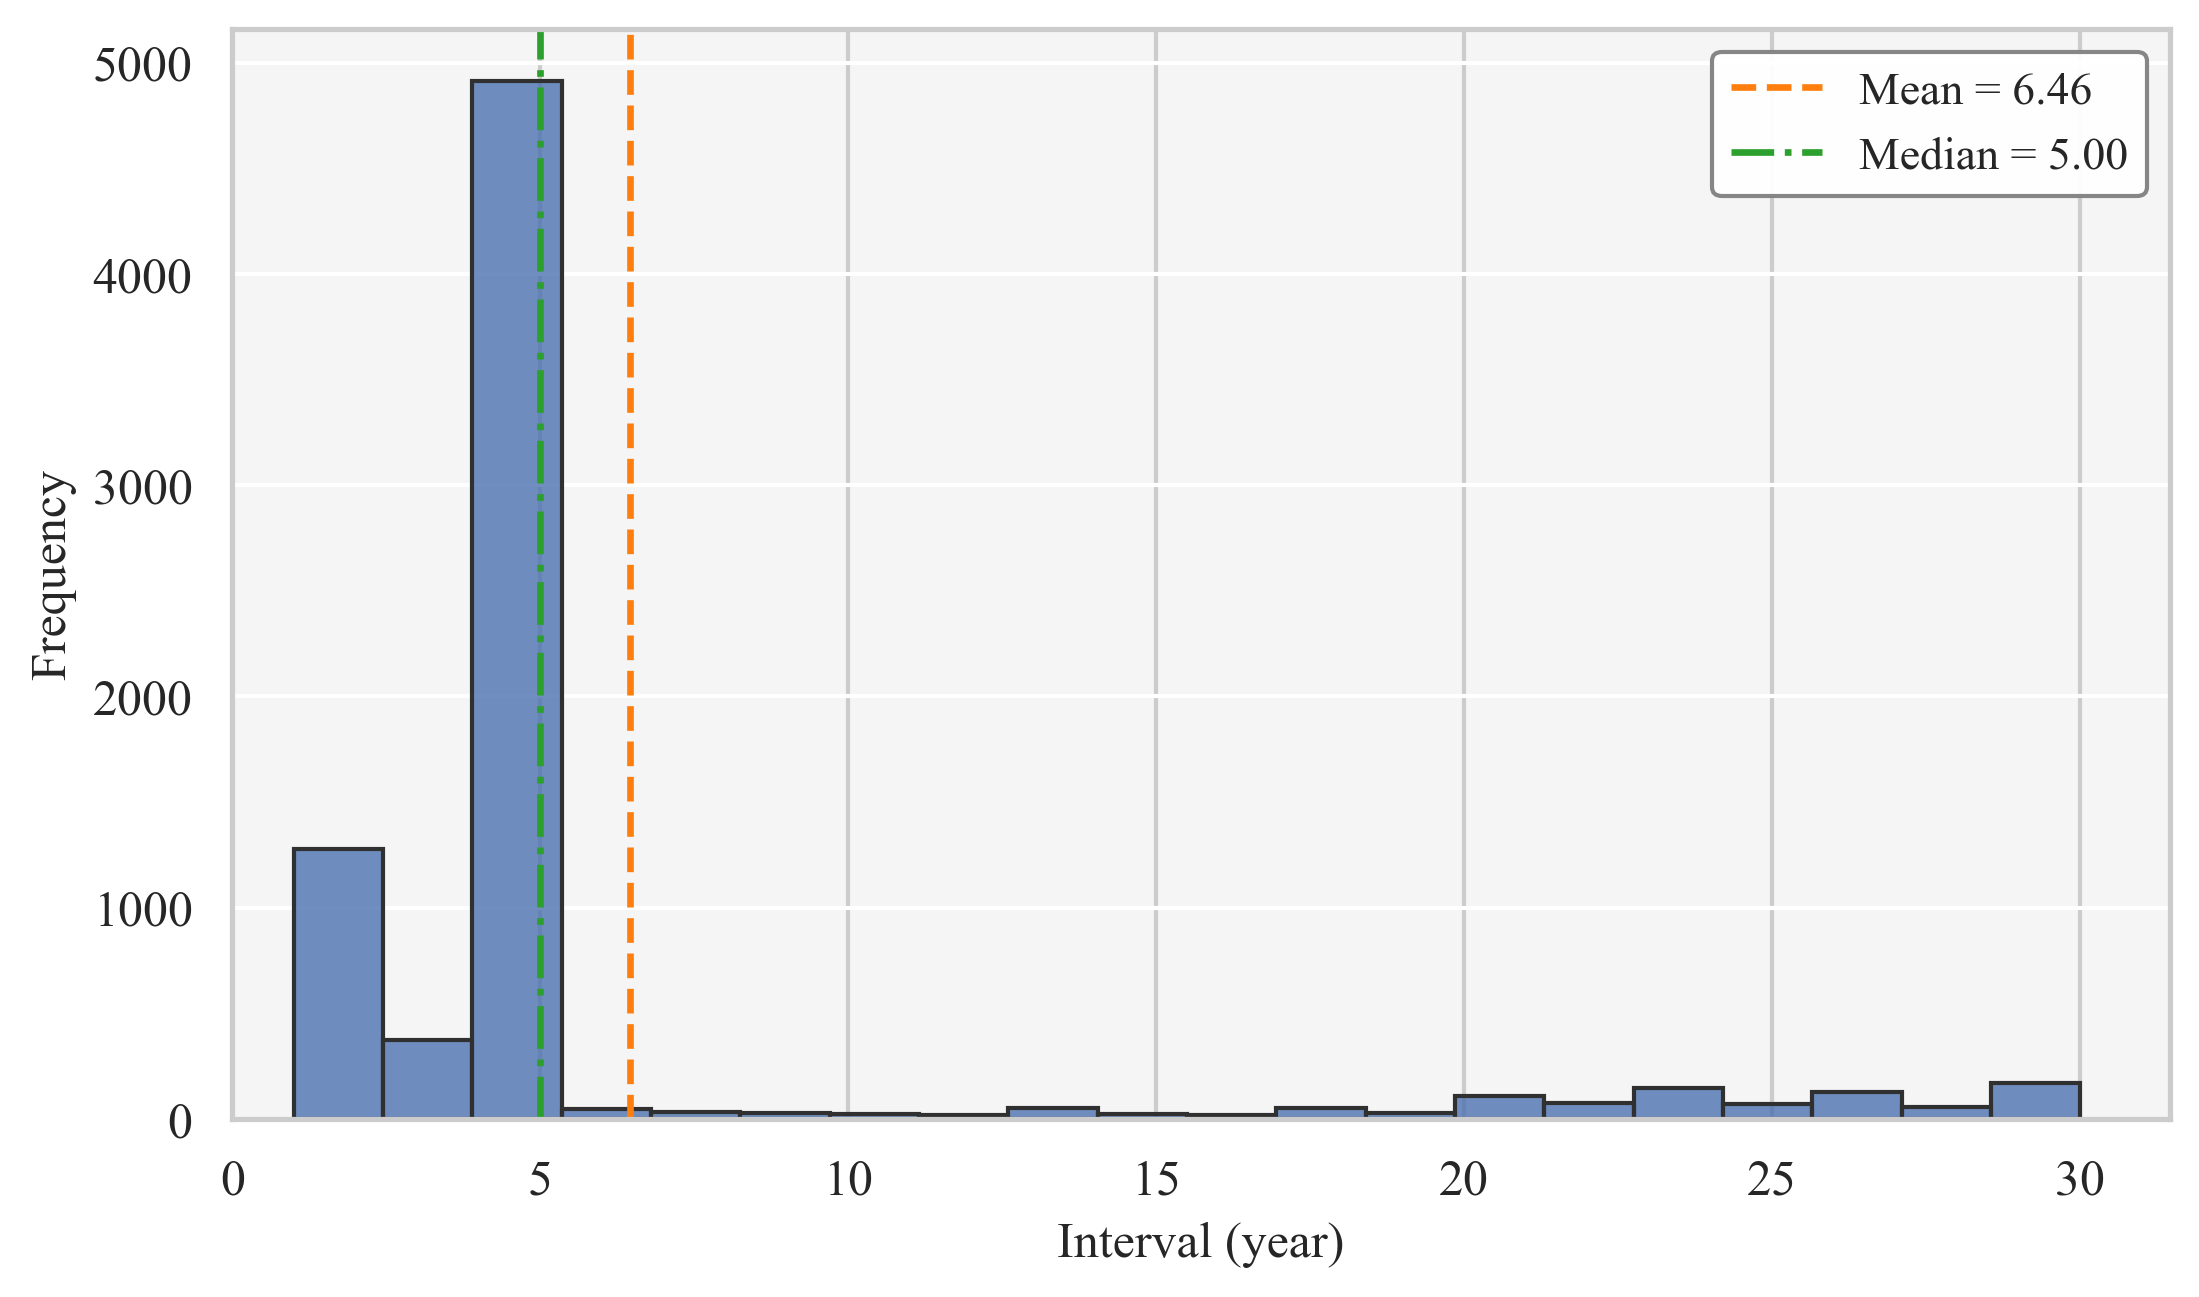
\includegraphics[width=0.75\linewidth]{figures/inspection_interval.png}
\caption{Distribution of inspection intervals used for transition-probability estimation.}
\label{fig:inspection_interval}
\end{figure}

\subsection{Estimated Transition Probabilities and Repair-Demand Probability}

前章で示したマルコフ劣化ハザードモデルを，前節の点検履歴へ適用した．本研究では説明変数を定数項のみとし，宮城県内RC橋に共通する1年間の推移確率行列を推定した．判定IVをIIIへ統合した3状態モデルの推移確率行列は，
\[
P =
\left(
\begin{array}{ccc}
0.9132 & 0.0862 & 0.0006 \\
0 & 0.9857 & 0.0143 \\
0 & 0 & 1
\end{array}
\right).
\]
となった．状態IIIを補修対象状態とし，補修後に状態Iへ回復する更新過程を仮定する．前章で定義した定常分布と補修状態への遷移確率の関係から，単一橋梁の定常状態における年間補修需要発生確率は，
\[
q=0.0123
\]
と得られる（約1.23\%）．以降の分析では，この値を対象322橋へ共通に適用する．

\subsection{Numerical Properties of the Expected Number of Contracts}

Figure~\ref{fig:expected_contracts_by_limit}は，推定した補修需要発生確率 \(q\) の下で，前章で導出した期待契約件数関数 \(f(N,L)\) を地域内橋梁数 \(N\) と同時発注上限 \(L\) の関数として計算した結果である．この図は，地域分割の効果が生じる基本的な機構を示す．\(L=1\) のとき，補修対象橋梁は個別に契約されるため，期待契約件数は \(Nq\) に等しい．これに対し，\(L>1\) では，同一地域・同一年度に発生した複数の補修需要を同一契約へ含められるため，\(N\) の増加に伴う期待契約件数の増加は小さくなる．

\begin{figure}[htbp]
\centering
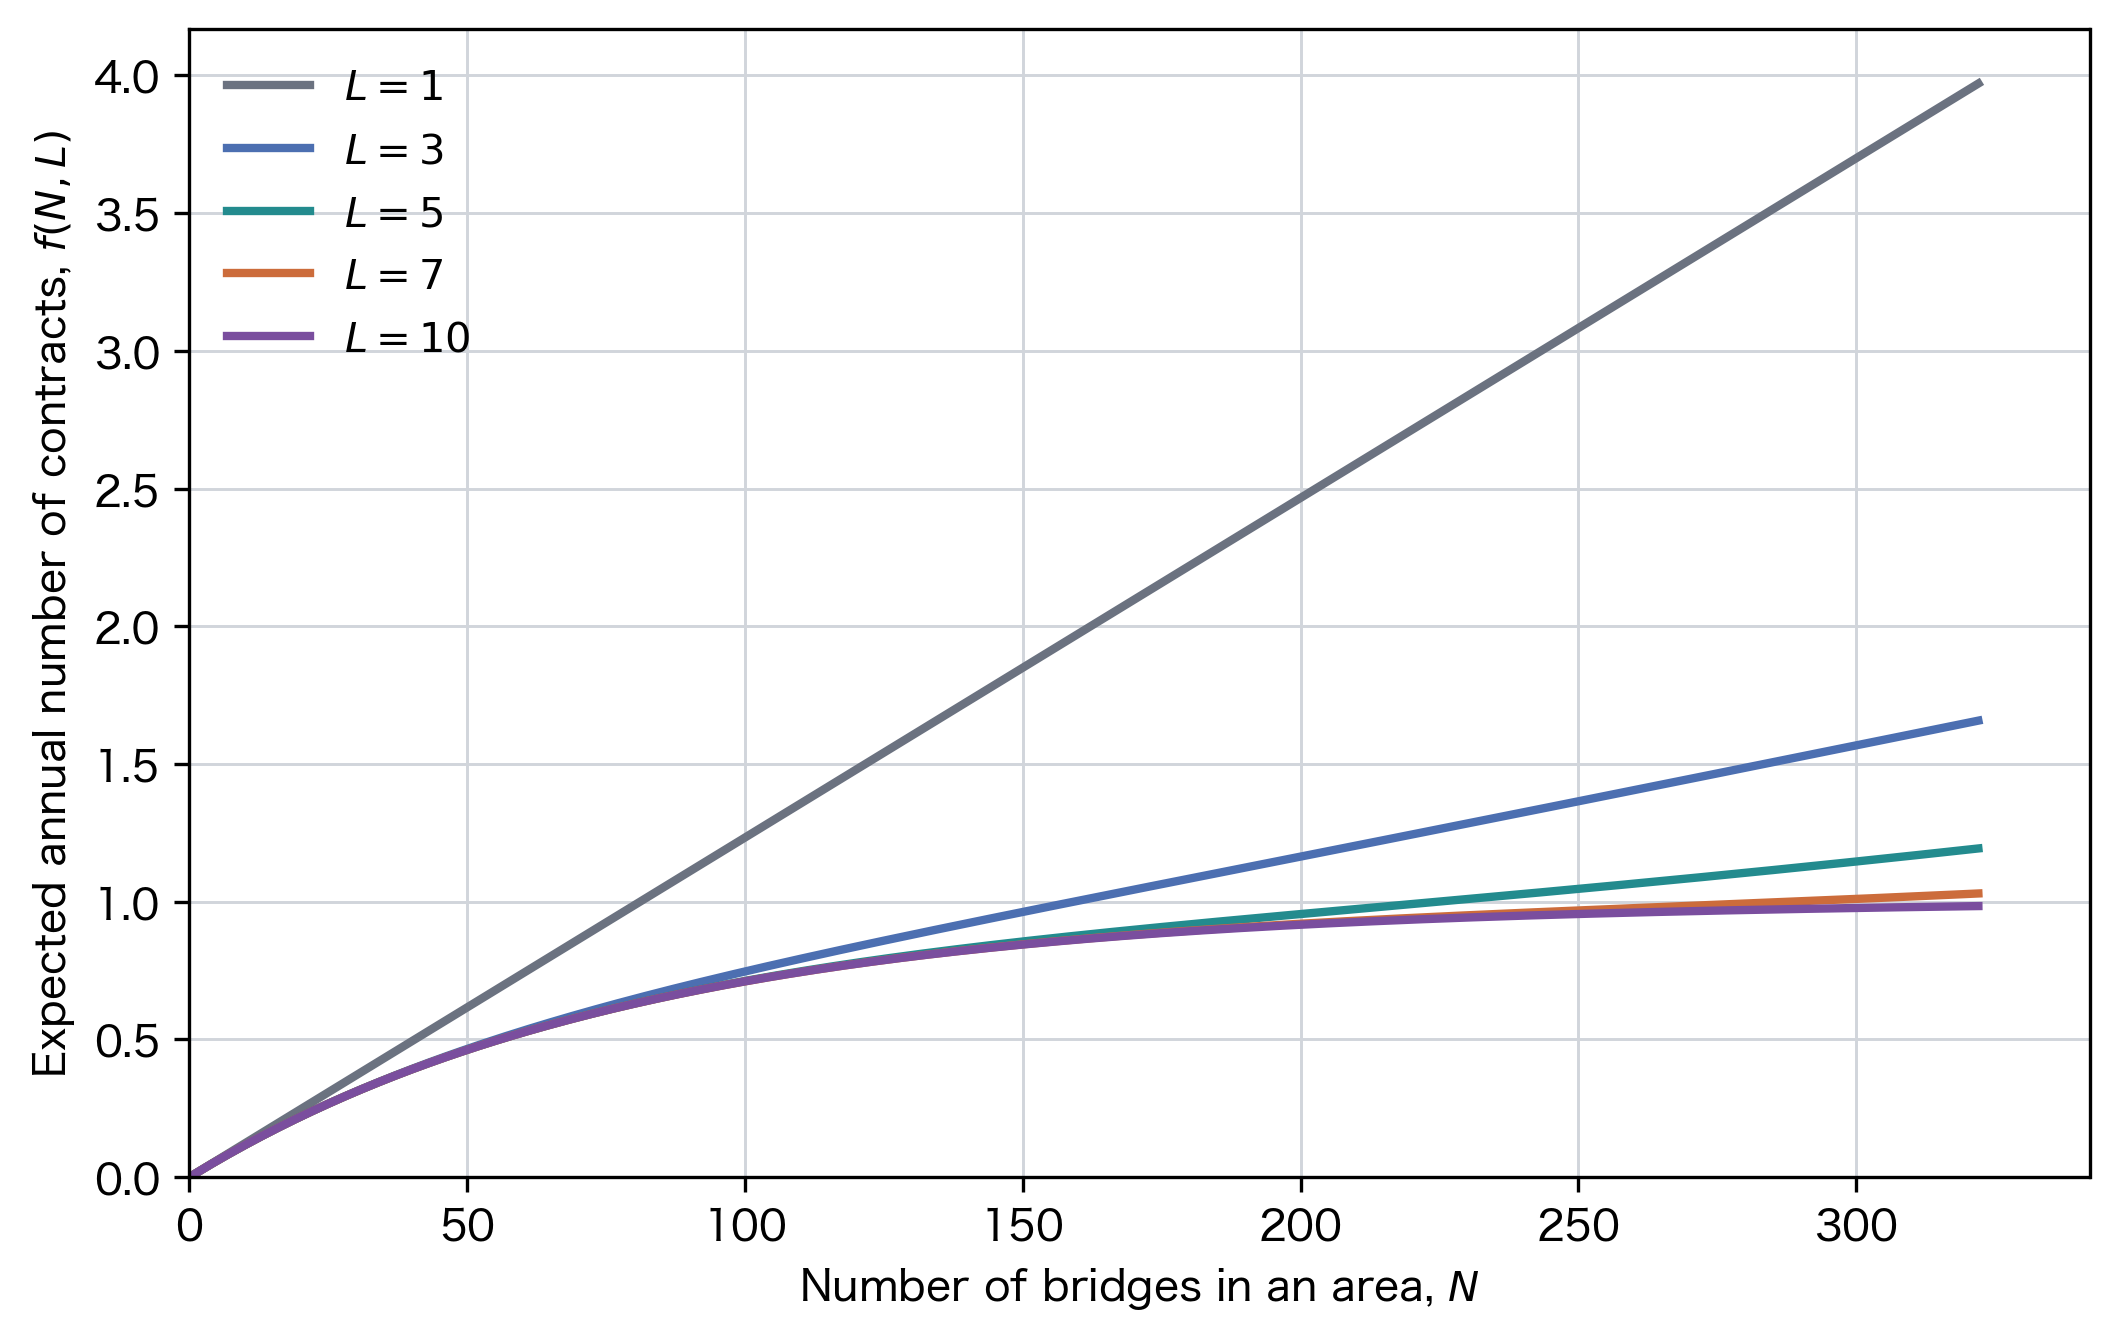
\includegraphics[width=0.78\linewidth]{figures/expected_contracts_by_bundle_limit.png}
\caption{Expected annual number of contracts \(f(N,L)\) by number of bridges \(N\) and bundling limit \(L\).}
\label{fig:expected_contracts_by_limit}
\end{figure}

特に，地域内橋梁数が小さい場合は，同一年度に複数の補修需要が生じる確率が低く，バンドリングの機会は限られる．一方，\(N\) が増えると複数の需要が同時に発生する可能性が高まり，\(L\) を大きく設定するほど期待契約件数を抑えられる．この関係が，複数の小規模管理主体の橋梁を同一の管理エリアに含めることによって契約集約効果が生じ得る理由を表している．

Figure~\ref{fig:expected_contracts_scaling}は，この機構を補足する．Figure~\ref{fig:expected_contracts_scaling}(a)は，同一地域内で年間に二つ以上の補修需要が発生する確率を示す．この事象が生じることが，複数案件を同一契約に集約する前提となる．\(N=322\) ではその確率は90.8\%である一方，\(N=50\) では12.7\%にとどまる．Figure~\ref{fig:expected_contracts_scaling}(b)は，個別発注（\(L=1\)）を基準とした期待契約件数の低減率を示す．主分析の \(L=5\) では，\(N=322\) における低減率は69.9\%である．ここでの低減率は個別発注との比較であり，現行の6市町による管理区分との比較とは基準が異なる．

\begin{figure}[htbp]
\centering
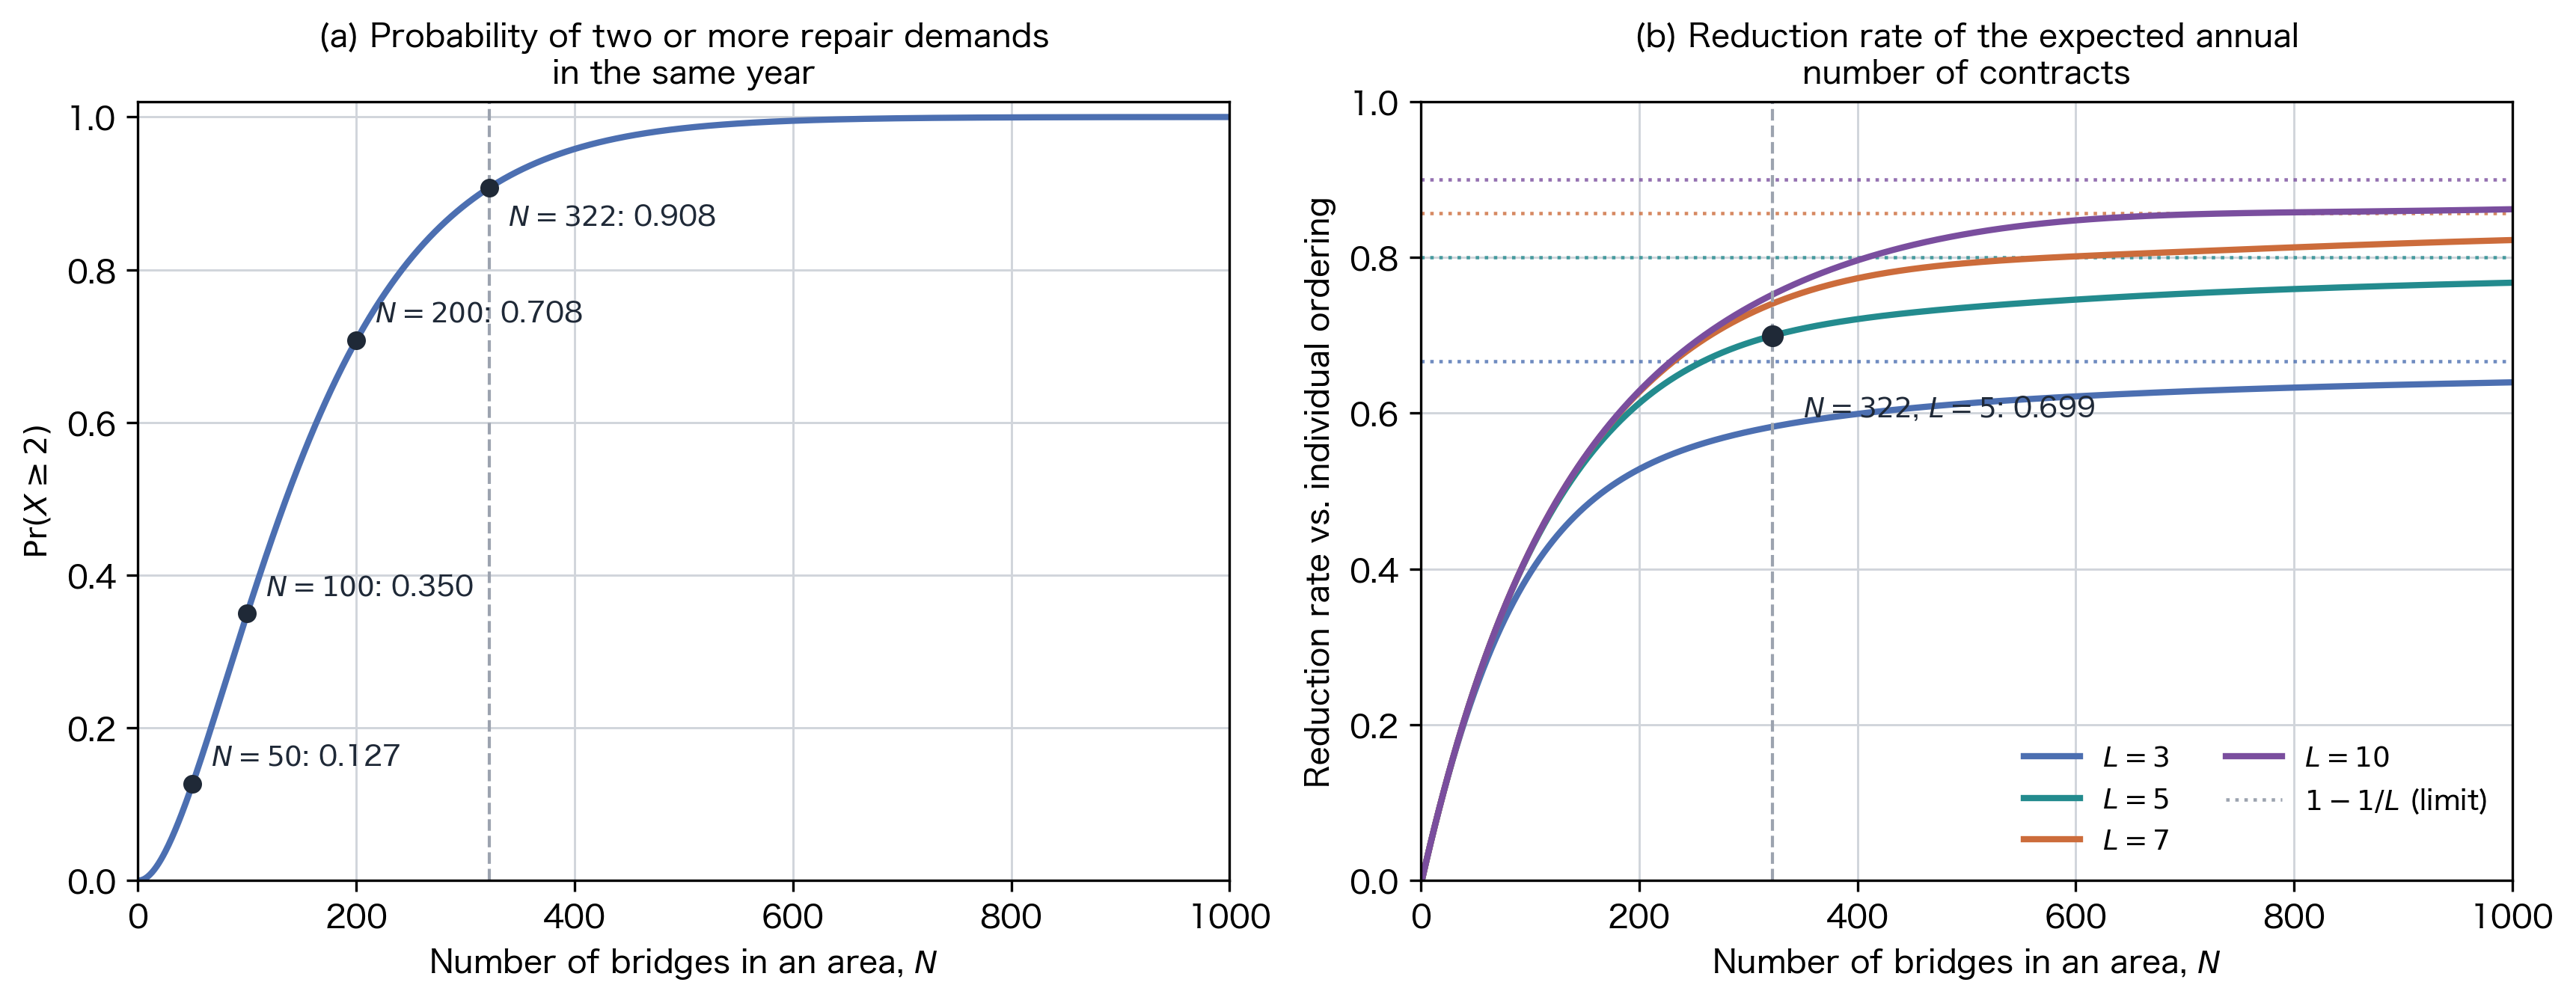
\includegraphics[width=0.92\linewidth]{figures/expected_contracts_scaling_analysis.png}
\caption{Conditions for bundling opportunities and reduction in expected contracts as the number of bridges in an area increases.}
\label{fig:expected_contracts_scaling}
\end{figure}

\subsection{Implementation and Analysis Settings}

地域分割最適化では，対象322橋を \(M\) 個の管理エリアへ割り当て，前章で定式化した期待契約件数の総和を最小化した．橋梁間距離には緯度・経度から算出した大円距離を用い，距離上限 \(D\) を管理エリアの地理的な広がりを表すシナリオパラメータとして設定した．主分析の同時発注上限は \(L=5\) とした．

比較基準として，対象6市町村の現行の管理者区分を6つの管理エリアとみなし，各管理者が管理する橋梁数に対する期待契約件数を合計した．同一の \(q\) および \(L\) により計算した現行管理の期待契約件数は2.5883件である．

期待契約件数関数は地域内橋梁数に関する非線形関数であるため，実装では各整数の橋梁数に対する関数値を区分線形関数として最適化ソルバーへ与える．本分析では，対象橋梁総数322橋までの全整数点を節点に用いるPWL表現を採用し，Pythonで実装した混合整数最適化問題をGurobi Optimizerで求解した．橋梁数は整数値のみを取るため，このPWL表現はすべての実行可能な橋梁数において前章の期待契約件数関数と一致する．

\subsection{Districting Optimization Results}

\subsubsection{Sensitivity to Distance Limit and Number of Districts}

Figure~\ref{fig:dm_sensitivity}は，距離上限 \(D\) と地域数 \(M\) のすべての可解ケースについて，年間期待契約件数を示したものである．破線は現行の6市町による管理区分を基準として計算した期待契約件数である．距離上限を緩和するにつれて，各地域数における期待契約件数は低下する．これは，より離れた橋梁を同一管理エリアに含めることで，契約バンドリングの候補が増えるためである．

地域数の影響は，距離上限と橋梁の空間分布の組合せに依存する．したがって，期待契約件数だけから地域数を一意に定めることはできない．本研究では，地域数を外生的なシナリオとして与え，距離上限と併せて地域分割案を比較する．

\begin{figure}[htbp]
\centering
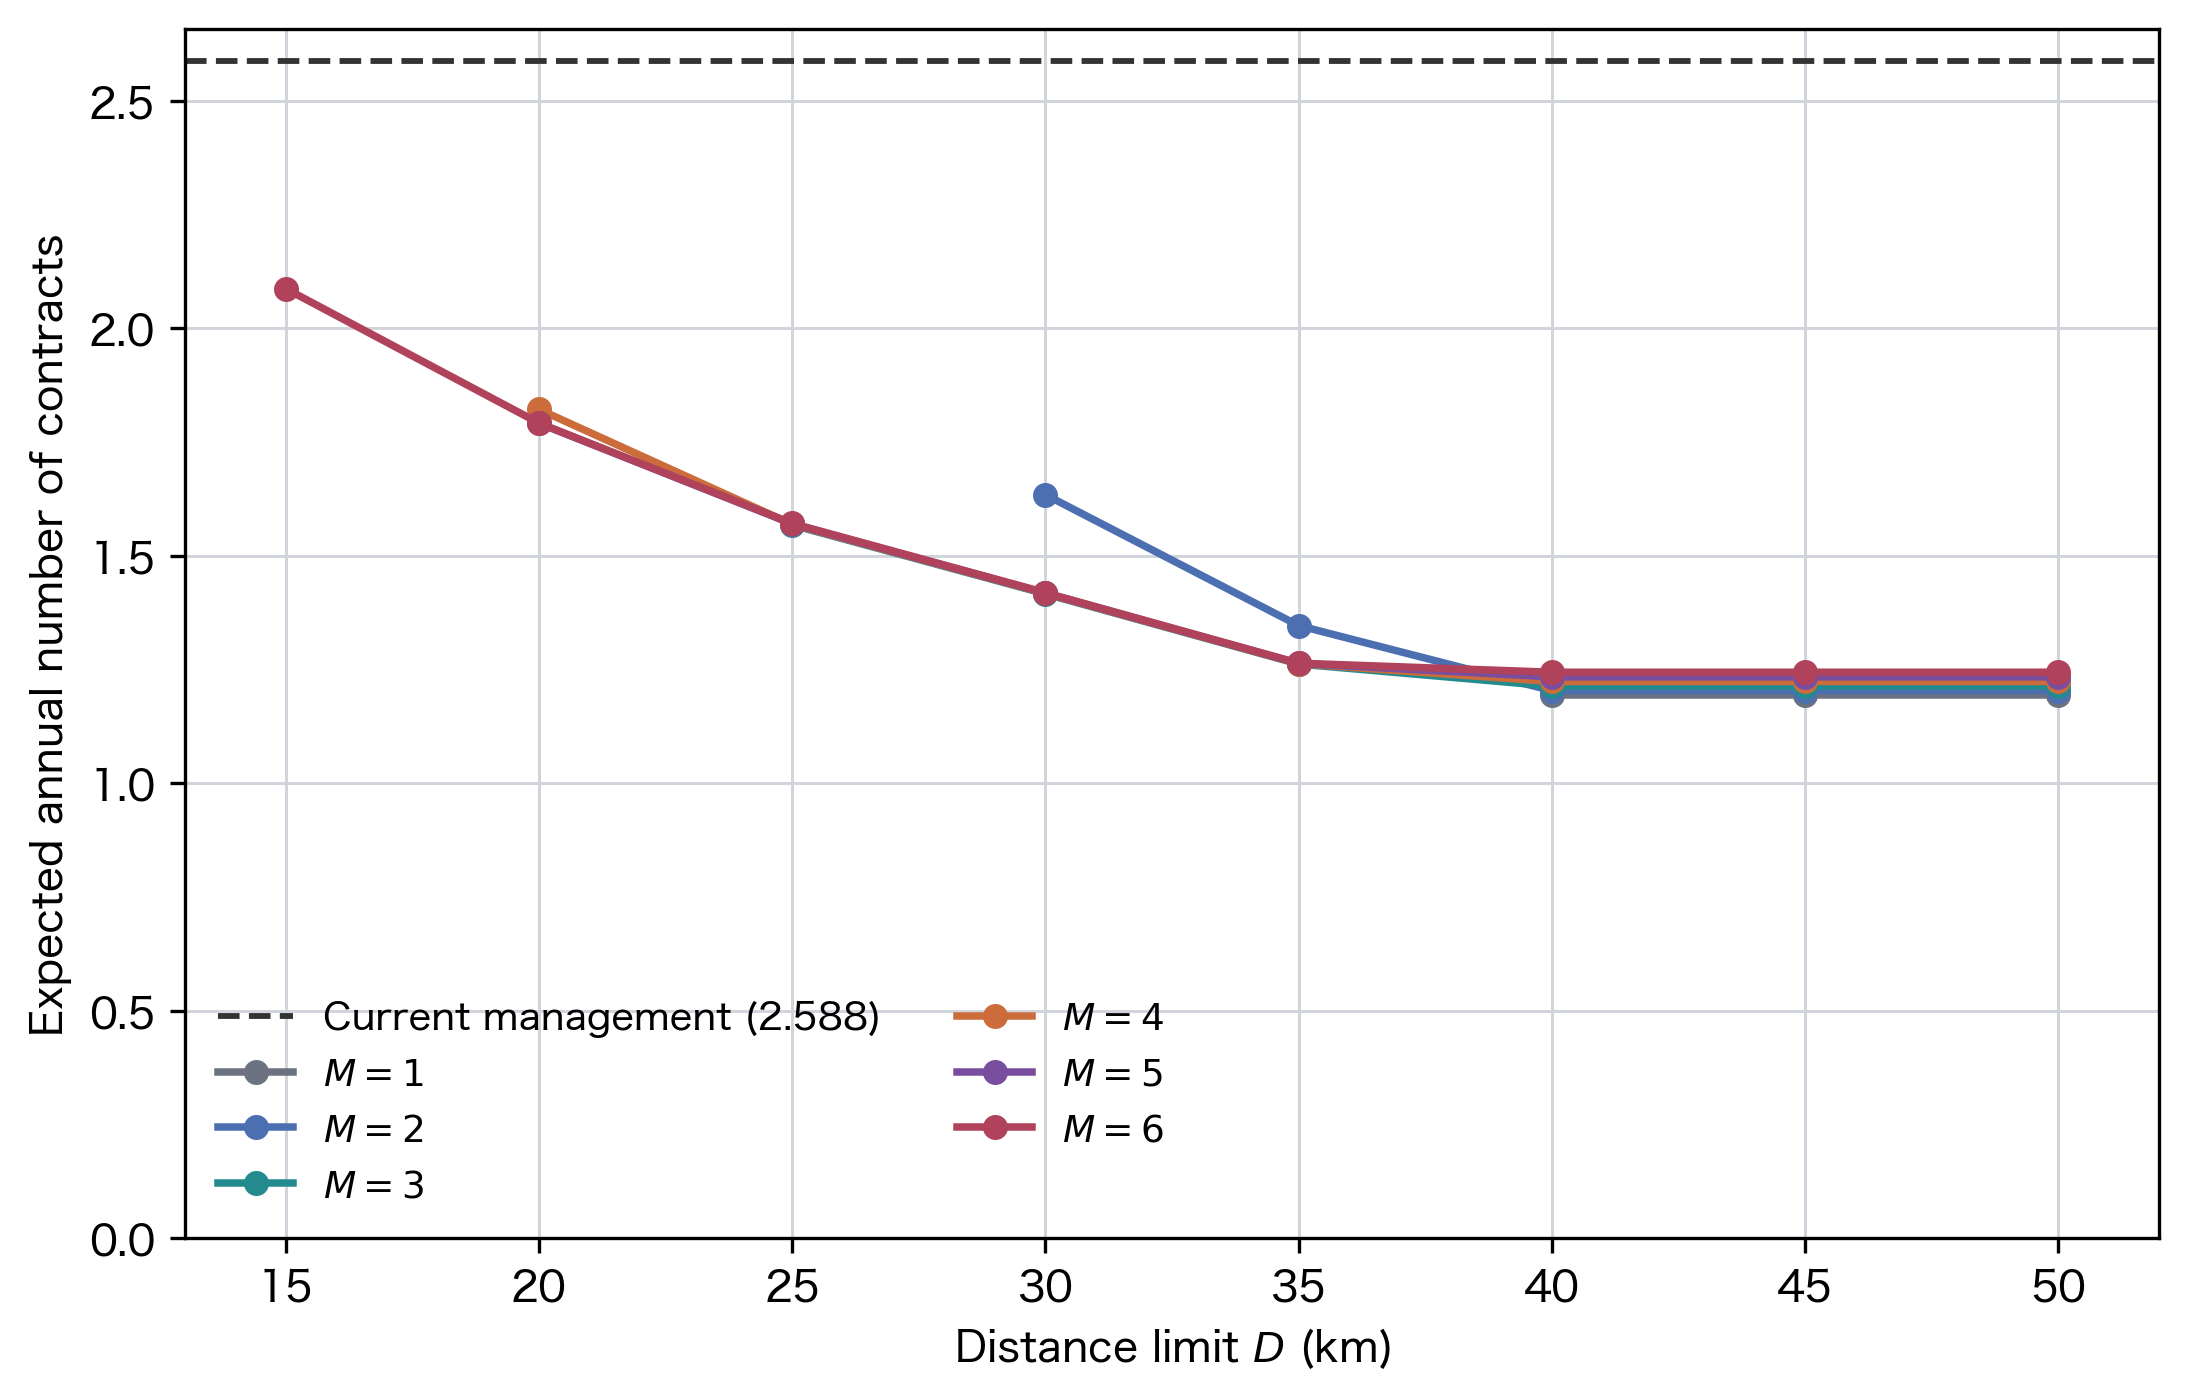
\includegraphics[width=0.82\linewidth]{figures/dm_sensitivity.png}
\caption{Expected annual number of contracts by distance limit \(D\) and number of districts \(M\).}
\label{fig:dm_sensitivity}
\end{figure}

Table~\ref{tab:optimization_results}には，各距離上限について期待契約件数が最小となる地域数を示す．距離上限を緩和するにつれて最小値は低下し，\(D\geq40\) kmでは全322橋を一つの管理エリアに含める解が得られる．このとき期待契約件数は1.1933件であり，現行管理と比べて53.9\%低い．

\begin{table}[htbp]
\centering
\caption{Comparison between current management and optimized districting solutions.}
\label{tab:optimization_results}
\begin{tabular}{lrr}
\toprule
Scenario & Expected contracts & Reduction from current management \\
\midrule
Current management & 2.5883 & 0.0\% \\
\(D=15\) km, \(M=6\) & 2.0871 & 19.4\% \\
\(D=20\) km, \(M=5\) & 1.7912 & 30.8\% \\
\(D=25\) km, \(M=3\) & 1.5677 & 39.4\% \\
\(D=30\) km, \(M=3\) & 1.4162 & 45.3\% \\
\(D=35\) km, \(M=3\) & 1.2620 & 51.2\% \\
\(D \geq 40\) km, \(M=1\) & 1.1933 & 53.9\% \\
\bottomrule
\end{tabular}
\end{table}

\subsubsection{District-Level Breakdown of Representative Solutions}

Figure~\ref{fig:region_breakdown}は，代表的な地域分割解について，各地域の橋梁数と期待契約件数への寄与を示す．\(D=25\) km，\(M=3\) では，橋梁数277，35および10の3地域が形成され，それぞれの期待契約件数は1.0987，0.3522および0.1167件である．\(D=35\) km，\(M=3\) では315橋を含む1地域と，6橋および1橋からなる小規模地域に分かれる．距離上限を40 kmまで緩和すると，322橋を一つの地域に含めることが可能となり，期待契約件数は1.1933件となる．

この内訳は，契約集約効果が単に地域数に依存するのではなく，大きな橋梁群を一つの地域に含められるかに強く依存することを示している．小規模地域が残る場合には，その地域でも補修需要に対応する契約単位が必要となるため，総期待契約件数は増加する．

\begin{figure}[htbp]
\centering
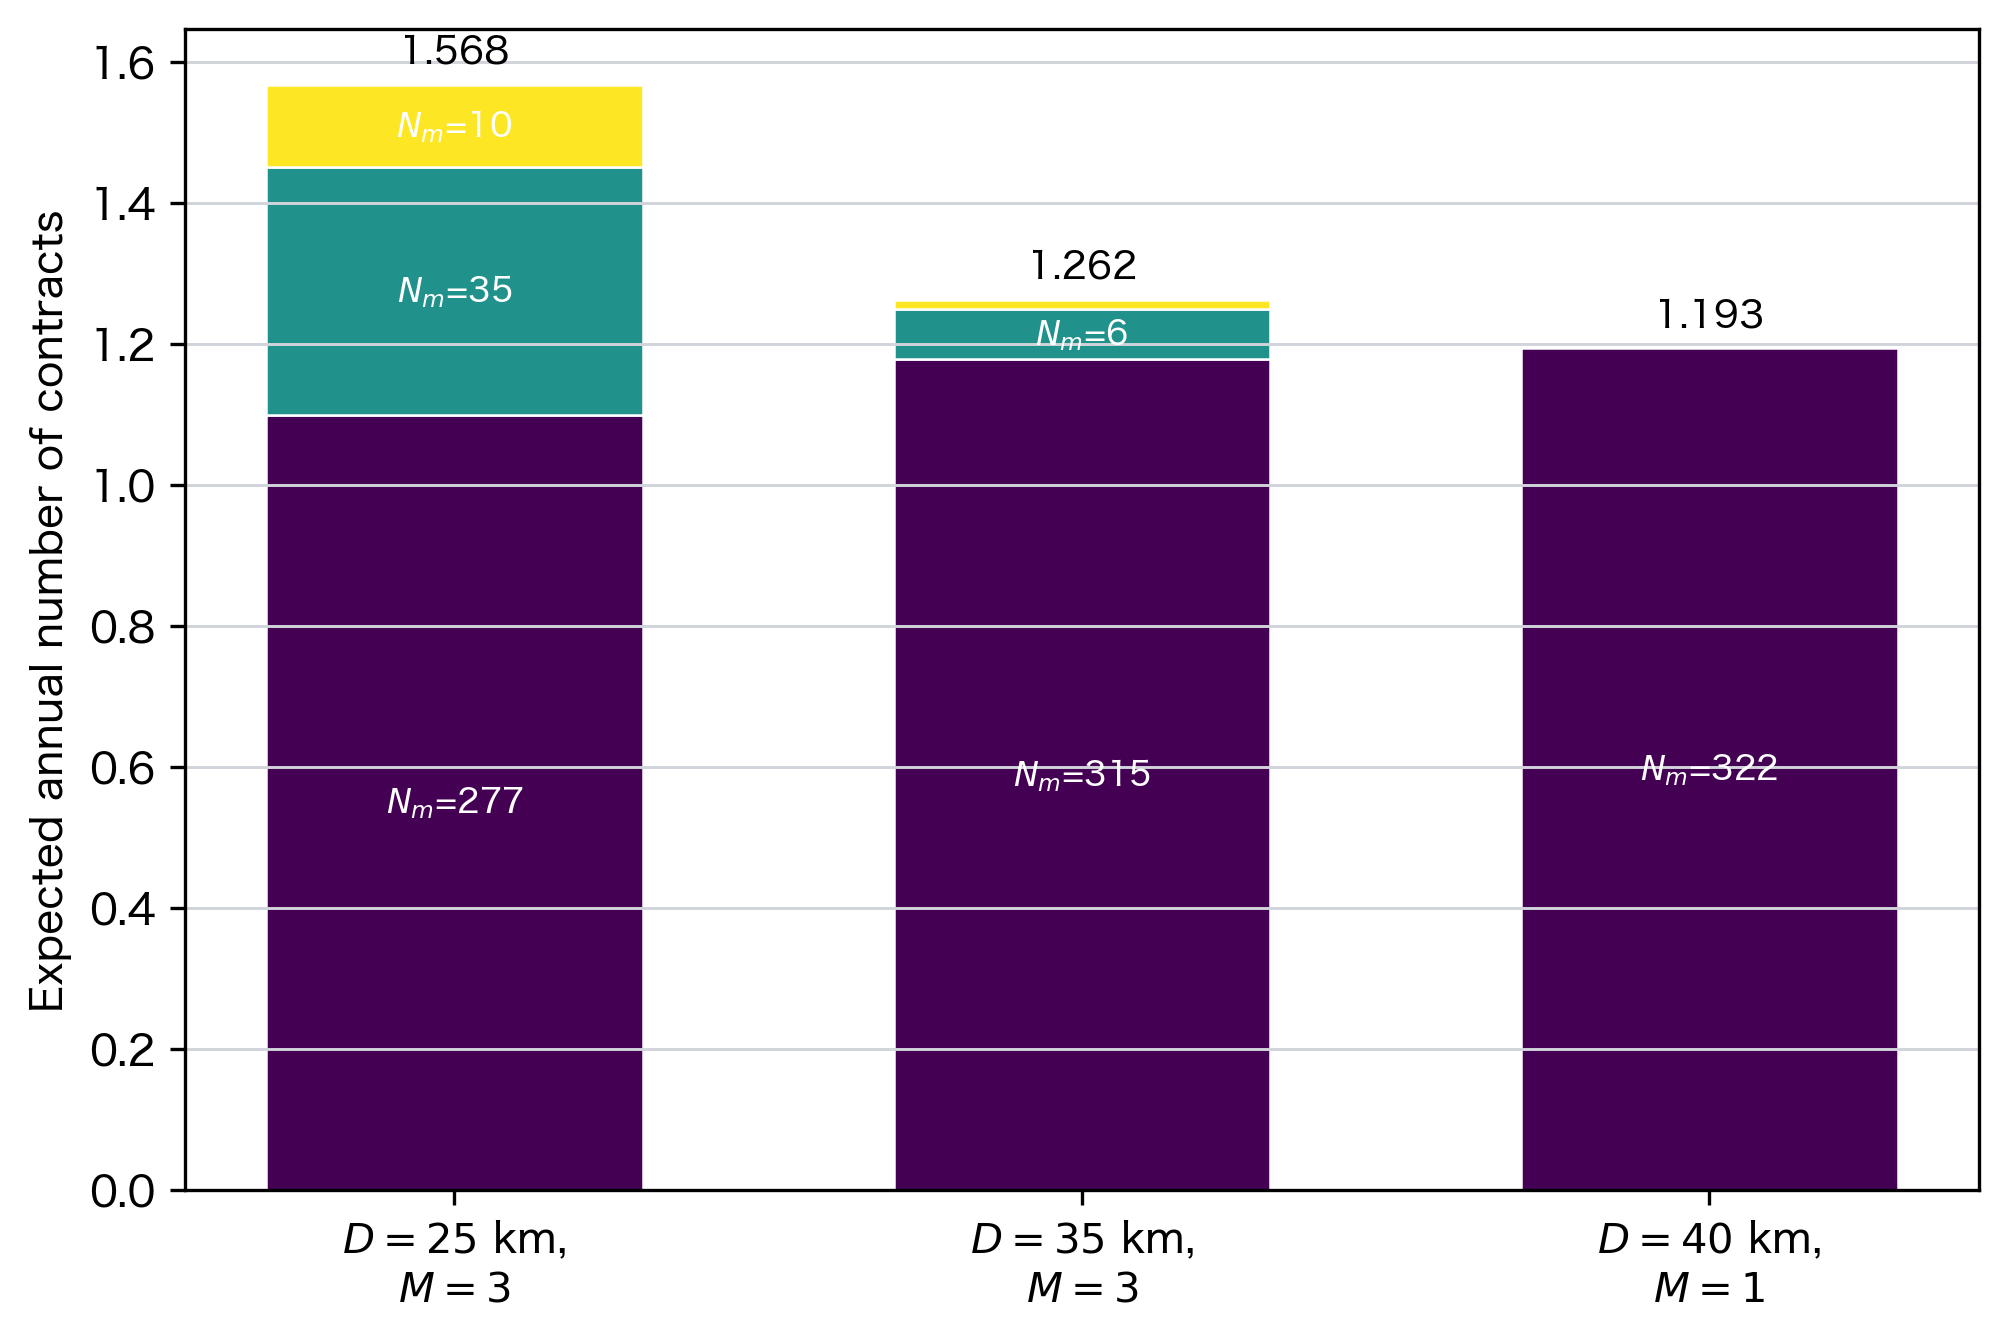
\includegraphics[width=0.82\linewidth]{figures/region_breakdown.png}
\caption{District-level breakdown of expected contracts for representative solutions.}
\label{fig:region_breakdown}
\end{figure}

\subsubsection{Spatial Configurations of Representative Solutions}

Figure~\ref{fig:districting_maps}は，前節で取り上げた3ケースの橋梁割当を地図上に示す．\(D=25\) km，\(M=3\) の解では，中央から南東部に広がる277橋の地域に加え，西部の10橋と北部から東部にかけての35橋が別地域となる．地域構成は現行の市町境界と必ずしも一致せず，複数の管理主体に属する橋梁を同一の発注対象候補としている．

\(D=35\) km，\(M=3\) では，大部分の315橋を一つの地域へ集約できる一方，地理的に周縁に位置する6橋および1橋は別地域となる．\(D=40\) km，\(M=1\) では，対象322橋が同一地域に割り当てられる．この比較は，距離上限の緩和によって，行政界ではなく橋梁間の空間的近接性に基づく集約が進むことを示している．

図中の面は，割り当てられた橋梁を基礎に作成したVoronoi分割であり，地域構成を視覚化するための補助表現である．本モデルが直接決定するのは各橋梁の地域への割当であり，連続した面としての管理区域境界を最適化するものではない．

\begin{figure}[htbp]
\centering
\begin{minipage}{0.49\linewidth}
\centering
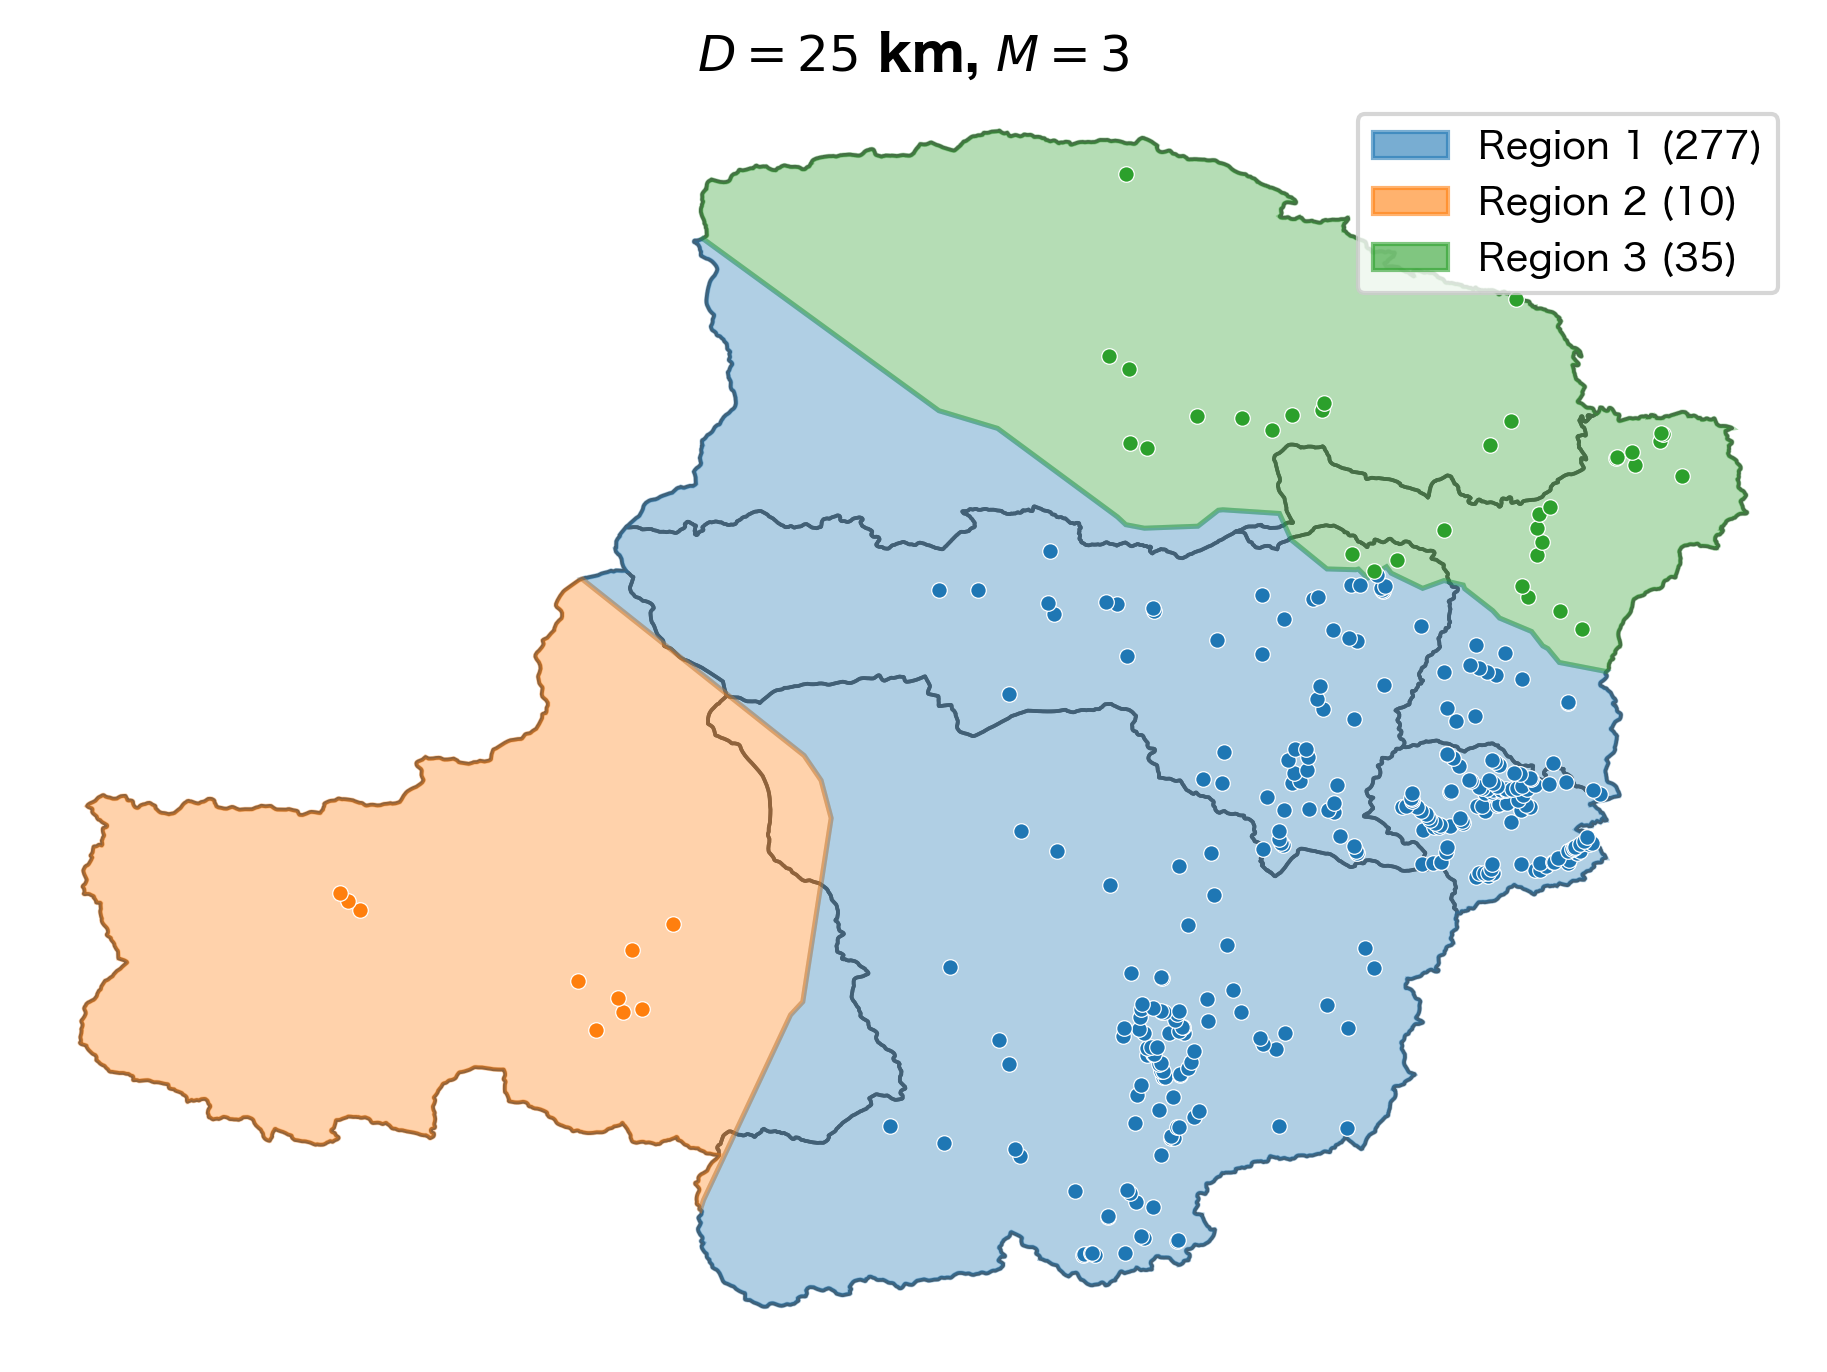
\includegraphics[width=\linewidth]{figures/districting_map_D25_M3.png}\\
(a) \(D=25\) km and \(M=3\).
\end{minipage}
\begin{minipage}{0.49\linewidth}
\centering
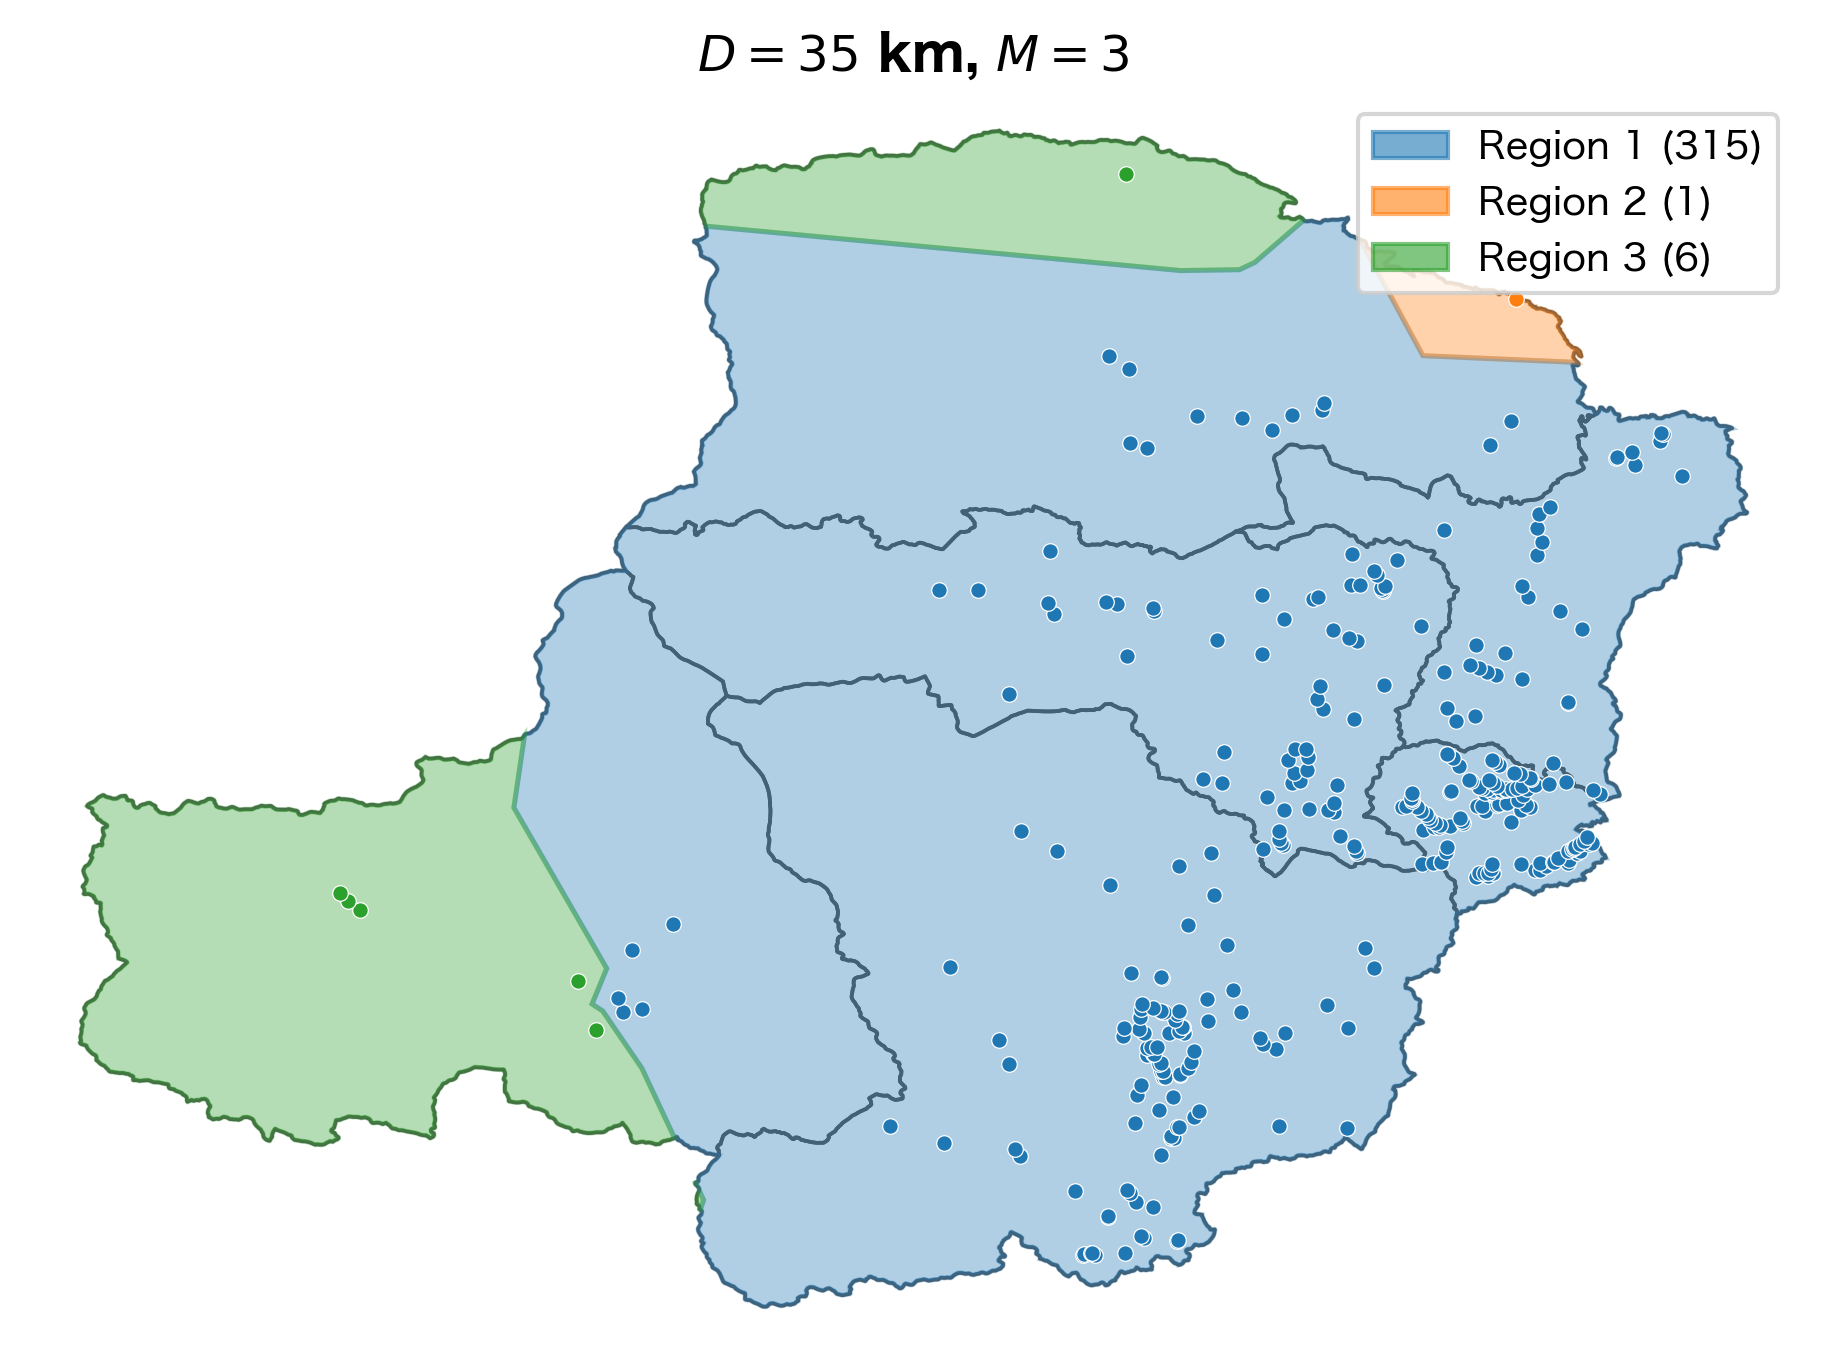
\includegraphics[width=\linewidth]{figures/districting_map_D35_M3.png}\\
(b) \(D=35\) km and \(M=3\).
\end{minipage}\\
\begin{minipage}{0.49\linewidth}
\centering
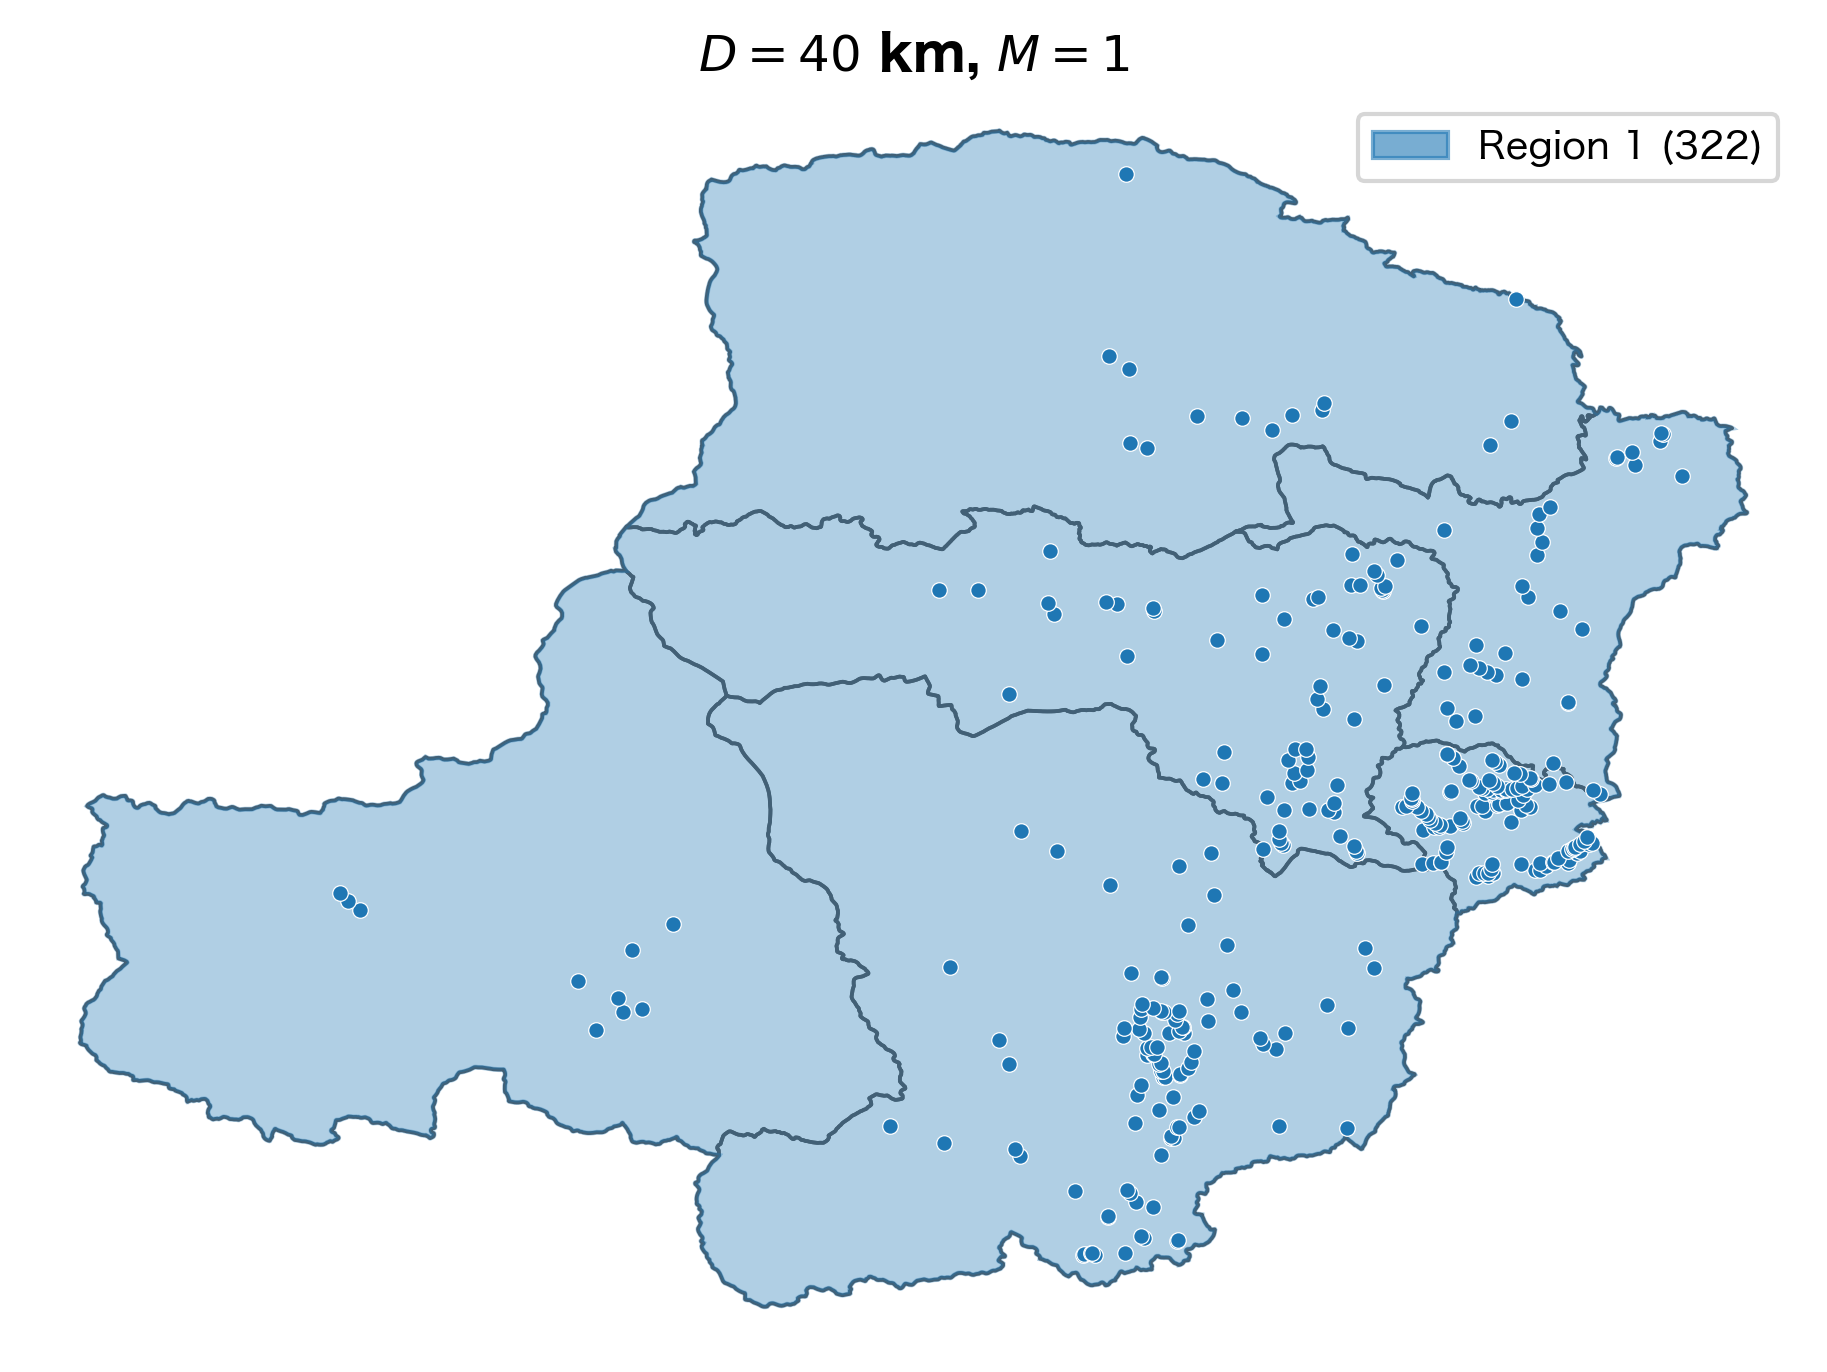
\includegraphics[width=\linewidth]{figures/districting_map_D40_M1.png}\\
(c) \(D=40\) km and \(M=1\).
\end{minipage}
\caption{Bridge assignments for representative distance limits and numbers of districts.}
\label{fig:districting_maps}
\end{figure}

全36ケースの地域割当地図は，Appendix Aに示す．

\section{Conclusions}

本研究では，広域連携による橋梁群の維持管理最適化に向けて，地域分割と集約効果を統合的に扱う混合整数計画モデルを構築した．マルコフ劣化モデルを用いた確率的補修需要の下で，地域に含まれる橋梁数ごとの期待契約件数を算定し，それを目的関数に組み込むことで，広域的な集約と地理的制約のトレードオフを定量的に評価した．

宮城県内の実橋梁データを対象とした数値解析の結果，地域数および距離上限の変化に応じて，発注効率の改善効果が確認された．また，現行の行政単位による管理体制と比較して，提案手法は期待契約件数を削減できる可能性を示した．

今後の課題としては，より実務的な契約一括化ロジックの反映，距離的要因以外の広域化による影響の定量化，より広域的地域スケールにおける最適化計算の実施，橋梁特性ごとのグルーピングが発注効率に及ぼす影響の分析などが挙げられる．

\begin{thebibliography}{99}
\bibitem{fhwafactsheet}
FHWA: Project Bundling Fact Sheet (EDC-5), Federal Highway Administration, U.S. Department of Transportation, 2020.
\bibitem{fhwa2019}
FHWA: Bridge Bundling Guidebook: An Efficient and Effective Method for Maintaining and Improving Bridge Assets, Federal Highway Administration, U.S. Department of Transportation, 2019.
\bibitem{mlit2025gunmane}
国土交通省：地域インフラ群再生戦略マネジメント手引き Ver.1，2025年10月.
\bibitem{nakazato2023}
Nakazato, Y., Mizutani, D. and Fukuyama, S.: Optimal Repair Policies for Infrastructure Systems with Life Cycle Cost Minimization and Annual Cost Leveling, Journal of Infrastructure Systems, Vol.29, No.3, 04023021, 2023. \url{https://doi.org/10.1061/JITSE4.ISENG-2169}
\bibitem{mizutani2025}
Mizutani, D., Fukuyama, S. and Satsukawa, K.: Optimal road facility spare parts location with continuum approximation, Transportation Research Part C: Emerging Technologies, Vol.174, 105109, 2025. \url{https://doi.org/10.1016/j.trc.2025.105109}
\bibitem{kalcsics2019}
Kalcsics, J. and Rios-Mercado, R. Z.: Districting Problems, Location Science, Springer International Publishing, pp.705--743, 2019.
\bibitem{qiao2026}
Qiao, J. Y., Guo, Y., Seilabi, S., Fricker, J. D. and Labi, S.: A proposed algorithm for identifying heuristic-optimal bundling strategies, Computer-Aided Civil and Infrastructure Engineering, Vol.49, 100100, 2026.
\bibitem{qiao2019}
Qiao, Y.: Bundling effects on contract performance of highway projects: quantitative analysis and optimization framework, Ph.D. Dissertation, Purdue University, 2019.
\bibitem{assaf2023}
Assaf, G. and Assaad, R. H.: Key decision-making factors influencing bundling strategies: analysis of bundled infrastructure projects, Journal of Infrastructure Systems, Vol.29, No.2, 2023.
\bibitem{assaf2024}
Assaf, G., Assaad, R. H. and Karaa, F.: Identifying the opportunities and challenges of project bundling: modeling and discovering key patterns using unsupervised machine learning, Journal of Infrastructure Systems, Vol.30, No.1, 2024.
\bibitem{gooijer2024}
Gooijer, N. J. C.: Entity-based System Dynamics for Bridge Asset Management: Exploring the Effects of Spatial Maintenance Cluster Strategies on Infrastructure System Performance, MSc Thesis, Delft University of Technology, 2024.
\bibitem{webster2013}
Webster, G. R.: Reflections on current criteria to evaluate redistricting plans, Political Geography, Vol.32, No.1, pp.3--14, 2013.
\bibitem{novaes2010}
Novaes, A. G. N., Frazzon, E. M., Scholz-Reiter, B. and Lima Jr., O. F.: A continuous districting model applied to logistics distribution problems, Proceedings of the XVI International Conference on Industrial Engineering and Operations Management, Sao Carlos, Brazil, 2010.
\bibitem{tsuda2005}
津田尚胤，貝戸清之，青木一也，小林潔司：橋梁劣化予測のためのマルコフ推移確率の推定，土木学会論文集，No.801/I-73，pp.69--82，2005.
\bibitem{roadstructuresdb}
全国道路施設点検データベース，\url{https://road-structures-db.mlit.go.jp}.
\bibitem{roadmaintenance}
道路メンテナンス年報 平成26年度--令和6年度，\url{https://www.mlit.go.jp/road/sisaku/yobohozen/yobohozen_maint_index.html}.
\bibitem{mlit2014inspection}
国土交通省：道路橋定期点検要領，2014年6月，\url{https://www.mlit.go.jp/common/001260174.pdf}.
\end{thebibliography}

\end{document}
